\subsection{Algèbre linéaire creuse}
\`{A} la différence de l'algèbre linéaire dense, la majorité des calculs faits en creux sont irréguliers.
%
C'est en partie dû à la façon de stocker la matrice creuse.
%
En effet, pour avoir un stockage efficace, seuls les coefficients non nuls de la matrice creuse sont stockés.
%
Le motif des valeurs non nulles de la matrice est défini par le problème que nous souhaitons résoudre.


Le format le plus générique pour stocker des matrices creuses s'appelle COO\footnote{COOrdinate list}.
%
Dans ce format, chaque valeur non nulle est stockée avec ses coordonnées 2D dans la matrice.
%
Ce format est souvent implémenté sous la forme de trois tableaux (Fig.~\ref{fig:COO}).
%
Chaque tableau s'occupera d'un propriété des éléments non nuls (valeur, colonne et ligne).
%
Toutes les matrices peuvent donc être représentées dans ce format.
%
Il peut être utile d'utiliser ce format lorsque nous souhaitons utiliser des algorithmes qui changent des valeurs nulles de la matrice en valeurs non nulles.
%
Mais ce format à l'inconvénient de ne pas imposer d'ordre sur les éléments de la matrice.
%
Il est donc difficile d'écrire un programme optimisé utilisant ce format.


\`A la place, un autre format est souvent utilisé, il s'agit du format CSR\footnote{Compress Sparse Row}.
%
Ce format permet lui aussi de stocker toutes sortes de matrices.
%
Il impose que les éléments non nuls soient rangés par ligne.
%
Il est aussi composé de trois tableaux et reprend deux des trois tableaux du format COO (valeur et colonne).
%
Le troisième tableau correspond aux indices de début et de fin de chaque ligne dans les deux autres tableaux (Fig.~\ref{fig:CSR}).
%
Ce troisième tableau peut être vu comme une compression du tableau indiçant les lignes de la matrice.
%
D'autres formats moins génériques existent, mais nous n'en parlerons pas ici.

\begin{figure}[!h]
     \begin{center}
        \subfigure[Exemple de matrice creuse]{%
            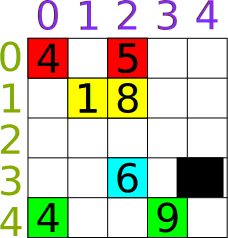
\includegraphics[width=0.25\textwidth]{matrix_format}
        }%
        \subfigure[Stockage COO]{%
           \label{fig:COO}
           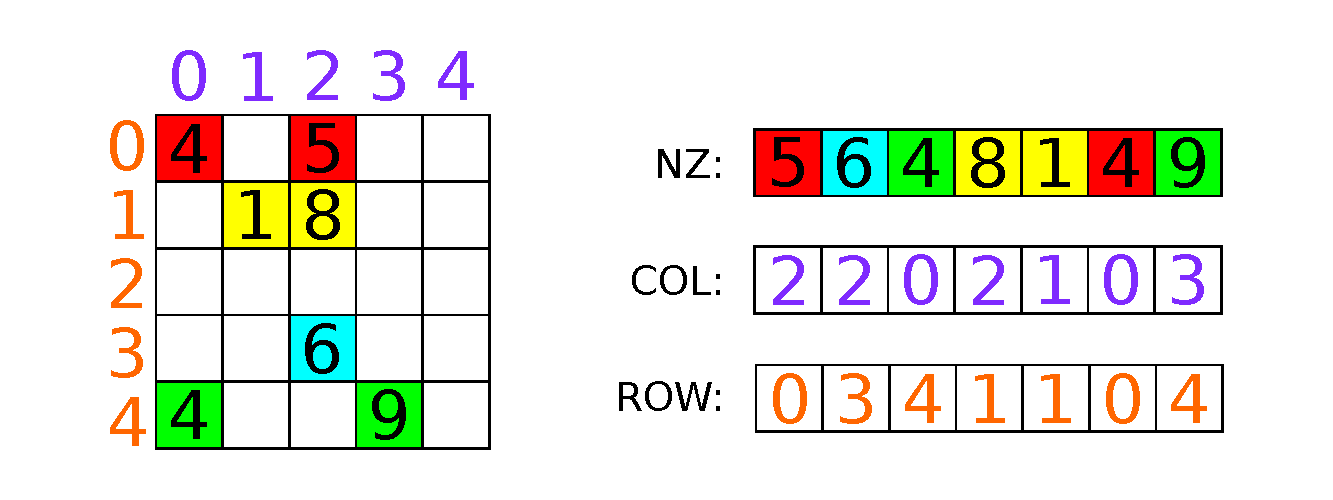
\includegraphics[width=0.35\textwidth]{COO}
        }%
        \subfigure[Stockage CSR]{%
            \label{fig:CSR}
            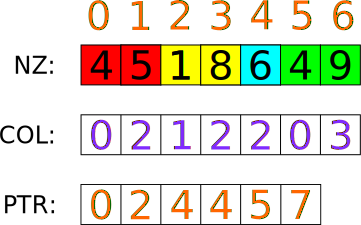
\includegraphics[width=0.35\textwidth]{CSR}
        }%
    \end{center}
    \caption{Comparaison entre les formats de stockage de matrices creuses COO et CSR.}
    \label{fig:matrix_storage}
\end{figure}


Le choix du format de stockage va avoir beaucoup d'effet sur les performances d'une application.
%
Avec la plupart des formats, nous aurons au moins deux accès mémoire pour obtenir les coordonnées 2D d'un coefficient non nul alors qu'avec l'algèbre linéaire dense nous pouvons calculer ces coordonnées à partir de la position dans la matrice.
%
Une partie non négligeable de la bande passante mémoire est donc utilisée juste pour la lecture des coordonnées 2D.
%
Les propriétés creuse et irrégulière de ces matrices impliquent aussi une mauvaise efficacité mémoire des noyaux d'algèbre linéaire creux à cause d'une mauvaise réutilisation du cache.
%
La plupart des optimisations faites en algèbre linéaire dense ne peuvent pas être appliquées à l'algèbre linéaire creuse à cause de l'irrégularité dans l'ordre des calculs ainsi que dans les accès mémoire.
%
Mais l'algèbre linéaire creuse nous permet de résoudre des problèmes bien plus grands que ceux qui utilisent l'algèbre linéaire dense.
%
Ceci est dû au fait qu'à ordre de matrice équivalente, une matrice creuse utilise vraiment moins de mémoire qu'une matrice dense.


Pour la simulation de réservoir, chaque entrée de nos matrices est composée d'un petit bloc dense dont la taille dépend du nombre de variables primaires utilisées par la simulation.
%
Nous reviendrons sur la définition de ces variables primaires plus loin dans ce document, disons qu'il s'agit du nombre de variables physiques simulées par cellule.
%
Ces blocs permettent d'obtenir une meilleure réutilisation des caches lors des opérations élémentaires (addition, multiplication ...).
%
Pour prendre en compte ces blocs et ainsi optimiser nos calculs, nous utilisons une version modifiée du CSR, le Block CSR ou BCSR.
%
La différence avec le format CSR provient du tableau servant stockant les valeurs non nulles de la matrice.
%
Au lieu de stocker des scalaires, nous stockons des blocs denses.
%
Ces blocs sont eux-mêmes stockés au format {\em column major}, ce qui signifie qu'en mémoire deux éléments consécutifs appartiennent à la même colonne.
%
Exception faite du dernier élément de la colonne dont l'élément consécutif est le premier élément de la colonne suivante.


Nous avons effectué une comparaison des différents formats de stockage des matrices appliqué au réservoir dans le cadre de l'utilisation d'un GPU, les résultats sont disponibles dans l'article~\cite{Renpar}.
%
Le format BCSR est un bon compromis entre flexibilité et performance.

Résoudre des problèmes linéaires creux est aussi très différent de résoudre des problèmes denses.
%
Nous ne pouvons pas utiliser une inversion directe de matrice, ou la technique de l'élimination de Gauss car la complexité en temps et en mémoire de ces méthodes est rédhibitoire pour nos applications.
%
De plus, nos problèmes ne nécessitent qu'une résolution approchée de la solution à chaque itération de l'algorithme de Newton.
%
Donc des méthodes différentes ont été inventées pour être capable de résoudre ces problèmes, beaucoup sont basées sur des méthodes itératives.
%
Nous démarrons donc avec une solution, ensuite ces méthodes réduisent itérativement la différence entre notre solution approximée et la solution réelle.
%
\`{A} la fin, nous obtenons une bonne approximation de la solution, ce qui est souvent suffisant pour être considéré comme la solution du problème.
